\section{Specification}
The algorithm for computing MRI-Q matrix is shown in Fig.~\ref{fig-1}. We want to accelerate the whole computation, mainly by loop unrolling and pipelining the inner for-loop. The programmer view algorithm C code and input dataset come from the Parboil benchmark suit~\cite{Rub1}. In this project, we will design accelerators which can accomodate the three datasets provided by Parboil benchmark, and make it capable of dealing with input images with arbitray size.


\subsection{Assessment}
We aim to design accelerators which can implement Q-matrix computation for any arbitrary input image sizes. The first goal is correctness. The Q-matrix computed by our accelerator should match the Q-matrix computed by software program. We calculate the difference between every output and its golden output, and deem it as a match when the difference is less than a certain threshold, otherwise it is an error. And we also set an error\_rate. If it is within a specified small value, we deem that our accelerator meet the correctness goal. The second goal is performance. We will measure the acceleration of our accelerator compared to its software execution running on FPGA board. We want our accelerators can be integrated with both Ariane core and Leon3 core. The generated RTL through Stratus HLS can be integrated and prototyped on FPGA. We will design both baremetal application and Linux application, the accelerator should pass both tests. At last we want to collect speedup data which indicates the acceleration effect. In achieving the second goal, we will do some amount of design space exploration, which includes designing accelerators with different area and latency trade-offs. 
\begin{figure}[t]
\centering
\captionsetup{justification=centering, format=hang}
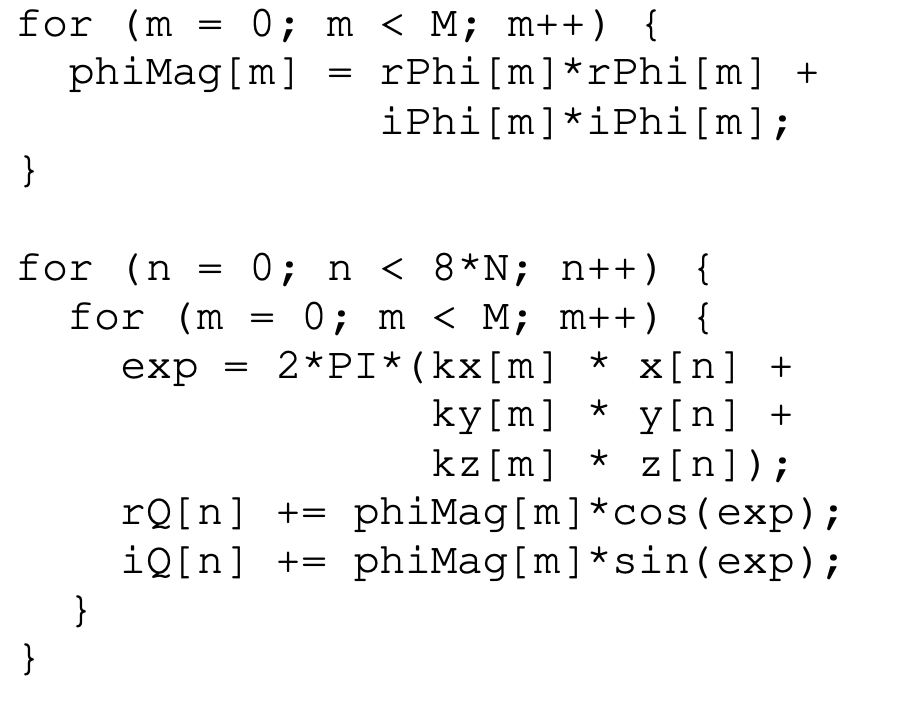
\includegraphics[width=0.85\columnwidth]{figures/algorithm-proposal.png}
\caption{Algorithm for computing MRI Q matrix~\cite{stone2008accelerating}}
\label{fig-1}
\end{figure}

\subsection{Milestones}\label{sec:arch}
\label{sec:milestones}

\vspace{-0.1in}
\begin{enumerate}
\setlength\itemsep{-0.15em}
  \item Analysis of the algorithm and the programmer's implementation in C (by Feb. 19)
  \item Learning two tutorials: "How to design an accelerator in SystemC (Cadence Stratus HLS)" and "How to design a single-core SoC"\cite{esp1}. (by Feb. 28)
  \item High-Level-Synthesis implementation in SystemC (by Mar. 11)
  \vspace{-2mm}
       \begin{itemize}
            \item Transform programmer view algorithm to HLS-ready SystemC
            \item Behavioral simulation
       \end{itemize}

  \item Baremetal application and linux application design. Evaluation on an FPGA platform (by Mar. 25)
  \item Mid-term presentation and report (by Mar. 25)
  \item Initial Design Space Exploration (by Apr. 15)
  \item Enhanced Design Space Exploration (by Apr. 22)
  \item Final refinement and analysis (by May 5)
  \item Design the same accelerator with Vivado HLS flow.
  \item Final presentation ($\sim$ May 11) and report ($\sim$ May 15)
\end{enumerate}

\subsection{Critical Aspects}
\begin{enumerate}
\setlength\itemsep{-0.15em}
\item Implement sine and cosine functions in for-loop.
\item Try different methods of optimization to reduce latency or decrease area.
\end{enumerate}
